\documentclass[12pt,a4paper]{report}

% =========================================================
% Packages
% =========================================================
\usepackage[a4paper,margin=2.5cm]{geometry}
\usepackage{graphicx}
\usepackage{xcolor}
\usepackage{setspace}
\usepackage{titlesec}
\usepackage{fancyhdr}
\usepackage{hyperref}
\usepackage{booktabs}
\usepackage{array}
\usepackage{longtable}
\usepackage{enumitem}
\usepackage{caption}
\usepackage{tikz}
\usepackage{circuitikz}
\usepackage{float}

\usetikzlibrary{arrows.meta, positioning, shapes.geometric, calc}

% =========================================================
% Colors and Formatting
% =========================================================
\definecolor{mainblue}{RGB}{20,55,105}
\definecolor{lightgray}{RGB}{245,245,245}
\definecolor{darkgray}{RGB}{70,70,70}

\hypersetup{
    colorlinks=true,
    linkcolor=mainblue,
    urlcolor=mainblue,
    citecolor=mainblue
}

\onehalfspacing

\titleformat{\chapter}
{\normalfont\huge\bfseries\color{mainblue}}
{\thechapter.}{1em}{}

\titleformat{\section}
{\normalfont\Large\bfseries\color{mainblue}}
{\thesection}{1em}{}

\titleformat{\subsection}
{\normalfont\large\bfseries\color{darkgray}}
{\thesubsection}{1em}{}

\pagestyle{fancy}
\fancyhf{}
\fancyhead[L]{SkyBit Circuit Project}
\fancyhead[R]{\thepage}
\renewcommand{\headrulewidth}{0.4pt}

% =========================================================
% Project Information
% =========================================================
\newcommand{\projectTitle}{SkyBit: Real-Time IoT Display and RGB Control System}
\newcommand{\studentName}{Mahros AL-Qabasy}
\newcommand{\studentID}{223106831}
\newcommand{\supervisorName}{Dr. Ashraf Wahba}
\newcommand{\universityName}{Galala University}
\newcommand{\apiURL}{https://skybit-api.mahros.dev/api/v1}
\newcommand{\frontendURL}{https://skybit.mahros.dev}

% =========================================================
% Document
% =========================================================
\begin{document}

% =========================================================
% Cover Page
% =========================================================
\begin{titlepage}
    \centering

    \vspace*{1cm}

    \IfFileExists{galala_logo.png}{
        \includegraphics[width=0.28\textwidth]{galala_logo.png}
    }{
        \fbox{
            \begin{minipage}{0.28\textwidth}
                \centering
                \vspace{1cm}
                Galala University Logo
                \vspace{1cm}
            \end{minipage}
        }
    }

    \vspace{1.5cm}

    {\Large \textbf{\universityName}}\\[0.5cm]

    {\Huge \textbf{\projectTitle}}\\[0.6cm]

    {\Large \textbf{Electric and Electronic Circuits Project Report}}\\[1.5cm]

    \begin{table}[H]
        \centering
        \renewcommand{\arraystretch}{1.5}
        \begin{tabular}{>{\bfseries}p{5cm} p{7cm}}
            Student Name: & \studentName \\
            Student ID: & \studentID \\
            Supervisor: & \supervisorName \\
            Academic Year: & Spring 2026 \\
        \end{tabular}
    \end{table}

    \vfill

    {\large \today}

\end{titlepage}

\tableofcontents
\newpage

% =========================================================
% Introduction
% =========================================================
\chapter{Introduction}

The \textbf{SkyBit} project is a small-scale Internet of Things system designed to control a physical circuit in real time through a web-based interface. The system consists of an ESP8266 microcontroller, an RGB LED module, and an I2C OLED screen module. The ESP8266 connects to a remote API through Wi-Fi and receives live control commands using WebSocket communication.

The purpose of this project is to demonstrate the relationship between hardware circuits, embedded software, backend APIs, and frontend web applications. The RGB LED module is used to represent color output, while the OLED screen is used to display dynamic text such as the word ``mahros'' or any text configured by the user from the web application.

This project is suitable for an electric and electronic circuits course because it combines basic electronic components, digital output control, serial communication concepts, I2C communication, and real-time software control.

% =========================================================
% Main Idea
% =========================================================
\chapter{Main Idea}

The main idea of SkyBit is to allow a user to control an electronic circuit remotely from a professional web interface. The frontend web application communicates with a backend API, and the backend API sends real-time updates to the ESP8266 module. The ESP8266 then updates the RGB LED color and the OLED screen content according to the received state.

The system has three main layers:

\begin{enumerate}[label=\textbf{\arabic*.}]
    \item \textbf{Hardware Layer:} ESP8266, RGB LED module, and OLED display.
    \item \textbf{API Layer:} Node.js backend server that stores and broadcasts the current device state.
    \item \textbf{Web Application Layer:} User interface that allows the user to configure LED color, screen text, display mode, and animation speed.
\end{enumerate}

The API acts as the central control point. The frontend sends configuration changes to the API, and the API immediately sends the updated state to the ESP8266 through a WebSocket connection.

% =========================================================
% Requirements
% =========================================================
\chapter{System Requirements}

\section{API Requirements}

The API is responsible for receiving control settings from the frontend, storing the current state, and broadcasting updates to the ESP8266 device.

\subsection{Functional Requirements}

\begin{longtable}{p{2.5cm} p{11cm}}
\toprule
\textbf{ID} & \textbf{Requirement} \\
\midrule
API-FR-01 & The API shall provide a health route to verify that the backend service is running. \\
API-FR-02 & The API shall expose a route to return the current system state. \\
API-FR-03 & The API shall expose a protected route to update the LED and screen state. \\
API-FR-04 & The API shall support WebSocket communication with the ESP8266 device. \\
API-FR-05 & The API shall send the latest state to the ESP8266 immediately after connection. \\
API-FR-06 & The API shall broadcast updated settings to the ESP8266 in real time. \\
API-FR-07 & The API shall validate LED values to be within the RGB range from 0 to 255. \\
API-FR-08 & The API shall validate screen text length to avoid memory issues on the ESP8266. \\
API-FR-09 & The API shall support basic authentication using a device token and an admin API key. \\
API-FR-10 & The API shall receive heartbeat/status messages from the ESP8266. \\
\bottomrule
\end{longtable}

\subsection{Non-Functional Requirements}

\begin{longtable}{p{2.5cm} p{11cm}}
\toprule
\textbf{ID} & \textbf{Requirement} \\
\midrule
API-NFR-01 & The API should respond to normal requests with low latency. \\
API-NFR-02 & The API should use HTTPS in production. \\
API-NFR-03 & The API should use secure WebSocket communication using WSS. \\
API-NFR-04 & The API should reject invalid JSON payloads. \\
API-NFR-05 & The API should use environment variables for sensitive configuration values. \\
API-NFR-06 & The API should limit request body size to reduce abuse risk. \\
API-NFR-07 & The API should be deployable behind a reverse proxy such as Nginx. \\
\bottomrule
\end{longtable}

\subsection{API Endpoints}

\begin{table}[H]
\centering
\renewcommand{\arraystretch}{1.4}
\begin{tabular}{p{3cm} p{5cm} p{6cm}}
\toprule
\textbf{Method} & \textbf{Endpoint} & \textbf{Purpose} \\
\midrule
GET & /api/v1/health & Checks API availability and connected clients. \\
GET & /api/v1/state & Returns the current LED and screen state. \\
PATCH & /api/v1/state & Updates the LED color and screen settings. \\
WS & /api/v1/device/ws & WebSocket channel used by the ESP8266. \\
WS & /api/v1/frontend/ws & Optional WebSocket channel used by the frontend. \\
\bottomrule
\end{tabular}
\caption{SkyBit API Endpoints}
\end{table}

\section{Web Application Requirements}

The web application is responsible for providing a professional user interface for controlling the hardware circuit.

\subsection{Functional Requirements}

\begin{longtable}{p{2.5cm} p{11cm}}
\toprule
\textbf{ID} & \textbf{Requirement} \\
\midrule
WEB-FR-01 & The web application shall allow the user to select the RGB LED color. \\
WEB-FR-02 & The web application shall allow the user to enter the text displayed on the OLED screen. \\
WEB-FR-03 & The web application shall allow the user to choose between static and scrolling text modes. \\
WEB-FR-04 & The web application shall allow the user to configure screen animation speed. \\
WEB-FR-05 & The web application shall allow the user to configure text size. \\
WEB-FR-06 & The web application shall send configuration updates to the API. \\
WEB-FR-07 & The web application shall display the current device state returned from the API. \\
WEB-FR-08 & The web application should show whether the device is connected or disconnected. \\
\bottomrule
\end{longtable}

\subsection{Non-Functional Requirements}

\begin{longtable}{p{2.5cm} p{11cm}}
\toprule
\textbf{ID} & \textbf{Requirement} \\
\midrule
WEB-NFR-01 & The interface should be responsive and usable on desktop and mobile screens. \\
WEB-NFR-02 & The interface should provide clear feedback after changing settings. \\
WEB-NFR-03 & The frontend should communicate only with the official API domain. \\
WEB-NFR-04 & The frontend should not expose sensitive backend secrets. \\
WEB-NFR-05 & The interface should be simple, professional, and suitable for demonstration. \\
\bottomrule
\end{longtable}

\section{Hardware Requirements}

The hardware layer is responsible for physically displaying the output controlled by the API.

\subsection{Components}

\begin{table}[H]
\centering
\renewcommand{\arraystretch}{1.4}
\begin{tabular}{p{5cm} p{8cm}}
\toprule
\textbf{Component} & \textbf{Purpose} \\
\midrule
ESP8266 NodeMCU Module & Main Wi-Fi microcontroller used to connect to the API and control outputs. \\
RGB LED Module with RGB- pins & Displays different colors based on API commands. \\
OLED I2C Screen Module & Displays text received from the API. \\
Jumper Wires & Used for circuit connections. \\
Breadboard & Used for temporary circuit assembly. \\
USB Cable & Used for power supply and firmware upload. \\
\bottomrule
\end{tabular}
\caption{Hardware Components}
\end{table}

\subsection{Functional Requirements}

\begin{longtable}{p{2.5cm} p{11cm}}
\toprule
\textbf{ID} & \textbf{Requirement} \\
\midrule
HW-FR-01 & The ESP8266 shall connect to a Wi-Fi network. \\
HW-FR-02 & The ESP8266 shall connect to the backend API using WebSocket. \\
HW-FR-03 & The ESP8266 shall control the red channel of the RGB LED. \\
HW-FR-04 & The ESP8266 shall control the green channel of the RGB LED. \\
HW-FR-05 & The ESP8266 shall control the blue channel of the RGB LED. \\
HW-FR-06 & The ESP8266 shall display text on the OLED screen using I2C communication. \\
HW-FR-07 & The ESP8266 shall support scrolling text animation on the screen. \\
HW-FR-08 & The ESP8266 shall send heartbeat/status messages to the API. \\
\bottomrule
\end{longtable}

\subsection{Non-Functional Requirements}

\begin{longtable}{p{2.5cm} p{11cm}}
\toprule
\textbf{ID} & \textbf{Requirement} \\
\midrule
HW-NFR-01 & The circuit should use safe ESP8266 GPIO pins that do not interfere with boot mode. \\
HW-NFR-02 & The OLED display should be powered using 3.3V unless its datasheet confirms 5V support. \\
HW-NFR-03 & The RGB LED module should use current-limiting resistors if they are not already included on the module. \\
HW-NFR-04 & The firmware should avoid blocking delays in the main loop where possible. \\
HW-NFR-05 & The ESP8266 should automatically reconnect to the WebSocket server if disconnected. \\
\bottomrule
\end{longtable}

% =========================================================
% Block Diagram
% =========================================================
\chapter{Block Diagram}

Figure~\ref{fig:block-diagram} shows the general stages of the SkyBit system.

\begin{figure}[H]
\centering
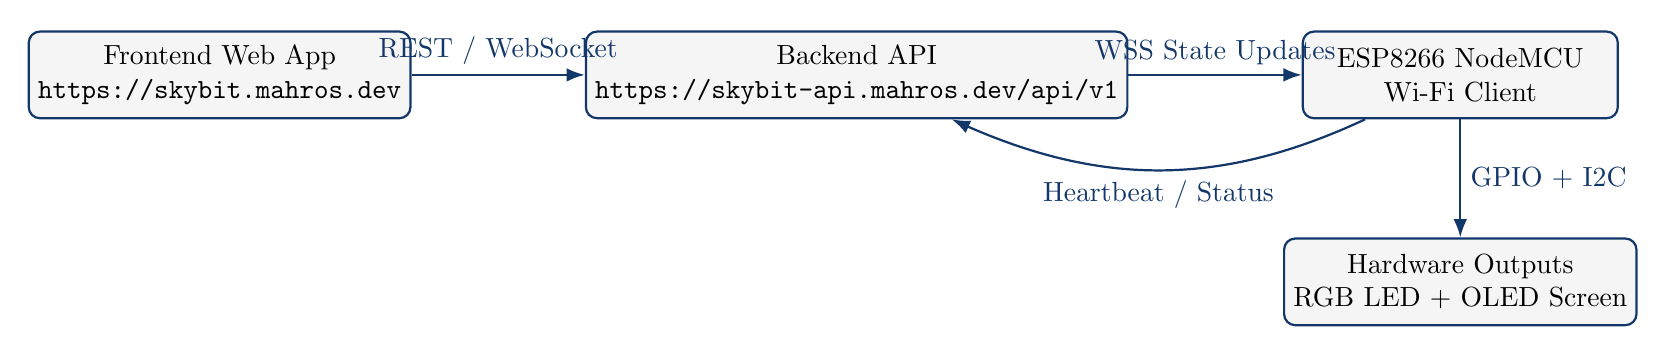
\begin{tikzpicture}[
    node distance=1.7cm,
    block/.style={
        rectangle,
        draw=mainblue,
        fill=lightgray,
        thick,
        rounded corners,
        minimum width=4cm,
        minimum height=1.1cm,
        align=center
    },
    arrow/.style={-Latex, thick, color=mainblue}
]

\node[block] (frontend) {Frontend Web App\\\texttt{\frontendURL}};
\node[block, right=2.2cm of frontend] (api) {Backend API\\\texttt{\apiURL}};
\node[block, right=2.2cm of api] (esp) {ESP8266 NodeMCU\\Wi-Fi Client};
\node[block, below=1.5cm of esp] (hardware) {Hardware Outputs\\RGB LED + OLED Screen};

\draw[arrow] (frontend) -- node[above]{REST / WebSocket} (api);
\draw[arrow] (api) -- node[above]{WSS State Updates} (esp);
\draw[arrow] (esp) -- node[right]{GPIO + I2C} (hardware);
\draw[arrow] (esp) to[bend left=25] node[below]{Heartbeat / Status} (api);

\end{tikzpicture}
\caption{General Block Diagram of the SkyBit System}
\label{fig:block-diagram}
\end{figure}

% =========================================================
% Circuit Diagram
% =========================================================
\chapter{Circuit Diagram}

The ESP8266 controls the RGB LED module using three digital PWM-capable GPIO pins. The OLED display is connected using the I2C protocol through SDA and SCL lines.

\section{Pin Connection Table}

\begin{table}[H]
\centering
\renewcommand{\arraystretch}{1.4}
\begin{tabular}{p{4cm} p{4cm} p{4cm}}
\toprule
\textbf{Module Pin} & \textbf{ESP8266 Pin} & \textbf{GPIO Number} \\
\midrule
RGB Red Pin & D5 & GPIO14 \\
RGB Green Pin & D6 & GPIO12 \\
RGB Blue Pin & D7 & GPIO13 \\
RGB Negative Pin & GND & GND \\
OLED GND & GND & GND \\
OLED VCC & 3V3 & 3.3V \\
OLED SCL & D1 & GPIO5 \\
OLED SDA & D2 & GPIO4 \\
\bottomrule
\end{tabular}
\caption{ESP8266 Pin Connections}
\end{table}

\section{Circuit Diagram}

\begin{figure}[H]
\centering
\begin{circuitikz}[american]

% ESP8266 block
\draw[thick, fill=lightgray] (0,0) rectangle (5,7);
\node at (2.5,6.6) {\textbf{ESP8266 NodeMCU}};

% ESP pins
\node[left] at (0,5.8) {3V3};
\node[left] at (0,5.2) {GND};
\node[left] at (0,4.6) {D1 / GPIO5};
\node[left] at (0,4.0) {D2 / GPIO4};

\node[right] at (5,5.8) {D5 / GPIO14};
\node[right] at (5,5.2) {D6 / GPIO12};
\node[right] at (5,4.6) {D7 / GPIO13};
\node[right] at (5,4.0) {GND};

% OLED block
\draw[thick, fill=lightgray] (-6,3.5) rectangle (-3,6.3);
\node at (-4.5,6.0) {\textbf{OLED I2C}};
\node[right] at (-6,5.5) {VCC};
\node[right] at (-6,5.0) {GND};
\node[right] at (-6,4.5) {SCL};
\node[right] at (-6,4.0) {SDA};

% RGB block
\draw[thick, fill=lightgray] (8,3.4) rectangle (11.5,6.3);
\node at (9.75,6.0) {\textbf{RGB LED Module}};
\node[left] at (11.5,5.4) {R};
\node[left] at (11.5,4.9) {G};
\node[left] at (11.5,4.4) {B};
\node[left] at (11.5,3.9) {-};

% OLED wires
\draw[mainblue, thick] (0,5.8) -- (-2,5.8) -- (-2,5.5) -- (-6,5.5);
\draw[mainblue, thick] (0,5.2) -- (-2.3,5.2) -- (-2.3,5.0) -- (-6,5.0);
\draw[mainblue, thick] (0,4.6) -- (-2.6,4.6) -- (-6,4.5);
\draw[mainblue, thick] (0,4.0) -- (-2.9,4.0) -- (-6,4.0);

% RGB wires
\draw[mainblue, thick] (5,5.8) -- (7,5.8) -- (7,5.4) -- (11.5,5.4);
\draw[mainblue, thick] (5,5.2) -- (7.3,5.2) -- (7.3,4.9) -- (11.5,4.9);
\draw[mainblue, thick] (5,4.6) -- (7.6,4.6) -- (7.6,4.4) -- (11.5,4.4);
\draw[mainblue, thick] (5,4.0) -- (7.9,4.0) -- (11.5,3.9);

\end{circuitikz}
\caption{Circuit Diagram for ESP8266, OLED Screen, and RGB LED Module}
\label{fig:circuit-diagram}
\end{figure}

% =========================================================
% Methodology
% =========================================================
\chapter{Methodology}

\section{Hardware Methodology}

The hardware circuit was assembled using an ESP8266 NodeMCU development board, one RGB LED module, and one OLED I2C display module. The RGB LED module was connected to GPIO14, GPIO12, and GPIO13 for red, green, and blue control respectively. The negative pin of the RGB module was connected to ground because the module is marked as RGB-, which indicates a common cathode configuration.

The OLED screen was connected using the I2C interface. The SCL pin was connected to GPIO5, and the SDA pin was connected to GPIO4. The display was powered from the 3.3V pin of the ESP8266.

\section{Firmware Methodology}

The ESP8266 firmware was developed using the Arduino IDE. The firmware performs the following tasks:

\begin{enumerate}
    \item Connects to the configured Wi-Fi network.
    \item Opens a secure WebSocket connection with the SkyBit API.
    \item Receives JSON messages that contain LED and screen settings.
    \item Updates the RGB LED color using PWM output.
    \item Displays text on the OLED screen.
    \item Animates the screen text when scroll mode is enabled.
    \item Sends heartbeat messages to the backend API.
\end{enumerate}

\section{API Methodology}

The backend API was designed using Node.js. It stores the current state of the system and provides REST endpoints for the frontend application. When the frontend updates the state, the API validates the request and broadcasts the new state to the ESP8266 through WebSocket communication.

The API state contains two main objects:

\begin{verbatim}
{
  "led": {
    "r": 255,
    "g": 0,
    "b": 0,
    "mode": "solid"
  },
  "screen": {
    "text": "mahros",
    "mode": "scroll",
    "speedMs": 30,
    "size": 2
  }
}
\end{verbatim}

\section{Web Application Methodology}

The web application provides a user-friendly control panel for the circuit. The user can select the LED color, write the text to be shown on the OLED screen, choose the screen display mode, and control animation speed. The frontend sends these settings to the API, which forwards them to the ESP8266 device.

% =========================================================
% Results
% =========================================================
\chapter{Results}

The project successfully demonstrates real-time control of a physical circuit using a web-based system. The ESP8266 module was able to connect to Wi-Fi and receive control messages from the backend API. The RGB LED module responded to color changes, and the OLED screen displayed the configured text.

The expected practical results are summarized as follows:

\begin{table}[H]
\centering
\renewcommand{\arraystretch}{1.4}
\begin{tabular}{p{5cm} p{8cm}}
\toprule
\textbf{Test Case} & \textbf{Result} \\
\midrule
ESP8266 firmware upload & Firmware uploaded successfully through Arduino IDE. \\
Wi-Fi connection & ESP8266 connects to the configured Wi-Fi network. \\
API health check & API returns service status successfully. \\
WebSocket connection & ESP8266 connects to the API through WebSocket. \\
RGB LED control & LED color changes according to API state. \\
OLED text display & OLED screen displays text received from API. \\
Scrolling text & Text moves across the OLED screen in scroll mode. \\
Frontend control & Web interface updates hardware settings through the API. \\
\bottomrule
\end{tabular}
\caption{Project Test Results}
\end{table}

The final system provides a complete connection between software and hardware. The frontend is responsible for user interaction, the API is responsible for state management and communication, and the ESP8266 is responsible for controlling the physical circuit.

% =========================================================
% Conclusion
% =========================================================
\chapter{Conclusion}

The SkyBit project demonstrates a practical real-time IoT system based on the ESP8266 microcontroller. The project combines electronic circuit design, embedded programming, backend development, and frontend web development into one integrated system.

The circuit uses a simple RGB LED module and an OLED screen, but the architecture can be extended to support more devices and sensors in the future. This makes the project a useful foundation for learning IoT systems, real-time communication, and hardware control through web technologies.

% =========================================================
% References
% =========================================================
\chapter{References}

\begin{thebibliography}{9}

\bibitem{esp8266}
Espressif Systems, \textit{ESP8266EX Datasheet}.  
Available: \url{https://www.espressif.com/}

\bibitem{arduino}
Arduino, \textit{Arduino Documentation}.  
Available: \url{https://docs.arduino.cc/}

\bibitem{websocket}
MDN Web Docs, \textit{The WebSocket API}.  
Available: \url{https://developer.mozilla.org/en-US/docs/Web/API/WebSockets_API}

\bibitem{nodejs}
Node.js, \textit{Node.js Documentation}.  
Available: \url{https://nodejs.org/en/docs}

\bibitem{ssd1306}
Adafruit, \textit{SSD1306 OLED Display Library Documentation}.  
Available: \url{https://github.com/adafruit/Adafruit_SSD1306}

\bibitem{arduinojson}
ArduinoJson, \textit{ArduinoJson Documentation}.  
Available: \url{https://arduinojson.org/}

\end{thebibliography}

\end{document}